\subsection{Perceptron classifier}
The perceptron forms part of the \textbf{artificial neural} network models, taking inspiration from the brain.

The perceptron is a basic processing element. It has inputs that may come from the environment (available data) or be the outputs of other perceptrons. Associated with each input, there is a \textit{connection weight}, and the output, in the simplest case, is a weighted sum of these inputs. However, in the most common case, this weighted sum is the input to an \textit{activation function} $f(x)$.

An intercept value $w_0$ is added to make the model more general and it can ba also thought of as a threshold value for the activation function. It is generally modeled as the weight coming from an extra \textit{bias unit} $x_0$ which is always $+1$. Thus, obtaining a simplified expression for the perceptron output $y$.
\begin{equation}
y = f({\boldsymbol{w}^T} \boldsymbol{x})
\end{equation}
where
\begin{equation*}
\begin{cases}
\boldsymbol{w} &= \begin{bmatrix} 	w_0 & w_1 & w_2 & \dots & w_d 	\end{bmatrix} \\
\boldsymbol{x} &= \begin{bmatrix} 	1 & x_1 & x_2 & \dots & x_d 	\end{bmatrix}
\end{cases}
\end{equation*}

The objective is to $learn$ the weights $\boldsymbol{w}$ such that correct outputs are generated given the inputs $\boldsymbol{x}$. If input is fed straight from the environment, a perceptron can be used to implement a linear fit; therefore it lies in the category of linear classifiers \cite{intro-2-ml-Alpaydm}.

\begin{figure}[]
	\centering
	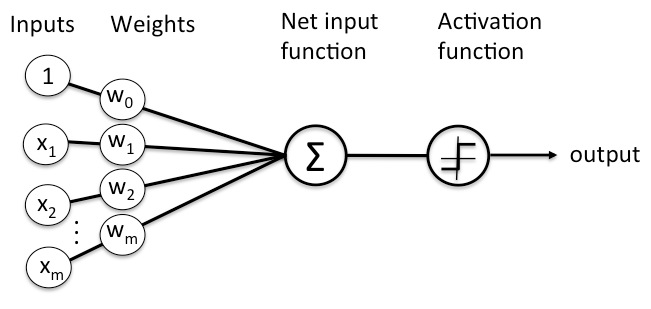
\includegraphics[width=0.4\paperwidth]{perceptron_schematic}
	\caption{Simple perceptron model}
	\label{fig:perceptron_schematic}
\end{figure}

\subsection{Cross-validation}
Training and testing a certain classifier model using the same data is a methodological mistake: a model that would just repeat the labels of previously seen samples will have a perfect score but fail to predict anything useful on yet unseen data. This situation is called \textbf{overfitting}. 

To avoid it, it is a common practice to hold out a part of the available data as a \textbf{test set}. Nonetheless, when evaluating different settings (\textit{hyper-parameters}) for classifiers, such as the $k$ value that must be manually set for the $k$-nn classifier, there is still a risk of overfitting on the test because the parameters can be tweaked until the classifier performs optimally.

To solve this problem, yet another part of the dataset can be held out as a so-called \textbf{validation set}. However, partitioning data into 3 sets drastically reduces the number of samples which can be used in the learning phase and results can depend on the random splitting of the sets.

A solution to this last problem is a procedure called \textbf{cross-validation} (CV for short). A test set should still be held out for final evaluation, but the validation set is no longer needed when doing CV. In the basic approach, the training set is split into $k$ smaller sets and the following procedure is followed for each of the $k$ \textit{folds}:
\begin{itemize}
	\item A model is trained using $k-1$ of the folds as training data.
	\item The remaining data is used as a test set to compute performance metrics (model validating).
\end{itemize}

The performance metric(s) reported by $k$-fold CV can then be averaged to obtain a more robust validation. This approach can be computationally expensive, but does not waste too much data \cite{scikit-learn}.

\begin{figure}[]
	\centering
	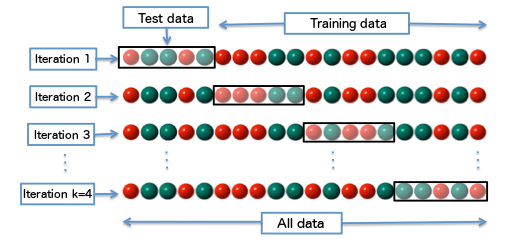
\includegraphics[width=0.4\paperwidth]{K-fold_cross_validation}
	\caption{$k$-fold cross validation diagram with $k=4$}
	\label{fig:k-fold_cross_validation}
\end{figure}
